\documentclass[border=4pt,12pt]{standalone}
% House style for redrawn exam diagrams (diagram-v4: 0.4pt lines, filled -latex arrows, fine dashes; stipple and hatching drawn as real dots/lines (no PDF/SVG patterns, so they render in every browser and at any scale); transparent background). Every figure \input's this.
\usepackage{amsmath,amssymb}
\usepackage{txfonts}
\usepackage{pdfrender,xcolor}
% \halo{text}: label on shading. The shading stops just around each letter's outline (a thin knock-out that follows the
% glyphs, like the papers' typesetting), never a box. Owner: "I don't want a box around the text".
\newcommand{\halo}[1]{\leavevmode\rlap{\pdfrender{TextRenderingMode=2,LineWidth=2.2pt,LineJoinStyle=1,StrokeColor=white,FillColor=white}#1}#1}
\usepackage{tikz,pgfplots}
\pgfplotsset{compat=1.18}
\usetikzlibrary{arrows.meta,calc,angles,quotes,patterns,patterns.meta,intersections,positioning,decorations.markings,shapes.geometric}
% Stipple and hatching are drawn as actual dots / lines clipped to the region (path picture), NOT as pattern fills:
% SVG <pattern> fills vanish or blur when browsers scale the image, so the owner could not see the shading.
% Each dot is a 0.72pt square (keeps SVGs small; reads as a dot at print size). Dots sit on one global staggered grid, so neighbouring regions line up.
\makeatletter
\newdimen\ex@x \newdimen\ex@y \newdimen\ex@xa \newdimen\ex@ya \newdimen\ex@xb \newdimen\ex@yb \newcount\ex@row
\def\exam@stipplecolor{black!75}\def\exam@dotr{0.42pt}\def\exam@dotgap{2.5}
\def\ex@rowdots{\ifdim\ex@x<\ex@xb \pgfpathrectangle{\pgfqpoint{\dimexpr\ex@x-0.36pt\relax}{\dimexpr\ex@y-0.36pt\relax}}{\pgfqpoint{0.72pt}{0.72pt}}\advance\ex@x by \exam@dotgap pt\relax\expandafter\ex@rowdots\fi}
\def\exam@stipple{%
  \pgftransformreset% dots are sized in real points even inside scaled pictures
  \pgfpointanchor{path picture bounding box}{south west}\ex@xa=\pgf@x \ex@ya=\pgf@y
  \pgfpointanchor{path picture bounding box}{north east}\ex@xb=\pgf@x \ex@yb=\pgf@y
  \pgfsetfillcolor{\exam@stipplecolor}\pgfmathsetmacro\ex@h{\exam@dotgap/2}%
  \pgfmathtruncatemacro\ex@r{floor(\ex@ya/\ex@h)-1}\ex@row=\ex@r\relax
  \ex@y=\ex@r\dimexpr\ex@h pt\relax
  \loop\ifdim\ex@y<\ex@yb
    \pgfmathtruncatemacro\ex@c{floor(\ex@xa/\exam@dotgap)-1}\ex@x=\ex@c\dimexpr\exam@dotgap pt\relax
    \ifodd\ex@row \advance\ex@x by \ex@h pt\fi
    \ex@rowdots
    \advance\ex@y by \ex@h pt \advance\ex@row by 1
    \ifnum\numexpr\ex@row-(\ex@row/4)*4\relax=0 \pgfusepath{fill}\fi% flush every 4 rows: bounded TeX memory, few clip copies in the SVG
  \repeat\pgfusepath{fill}}
\newdimen\ex@d
\def\exam@hatch#1{% #1 = 1 for /, -1 for \ ; lines 45 degrees, 3pt apart
  \pgftransformreset
  \pgfpointanchor{path picture bounding box}{south west}\ex@xa=\pgf@x \ex@ya=\pgf@y
  \pgfpointanchor{path picture bounding box}{north east}\ex@xb=\pgf@x \ex@yb=\pgf@y
  \ex@d=\dimexpr\ex@yb-\ex@ya\relax \ex@x=\dimexpr\ex@xa-\ex@d\relax
  \loop\ifdim\ex@x<\ex@xb
    \ifnum#1>0 \pgfpathmoveto{\pgfqpoint{\ex@x}{\ex@ya}}\pgfpathlineto{\pgfqpoint{\dimexpr\ex@x+\ex@d\relax}{\ex@yb}}%
    \else \pgfpathmoveto{\pgfqpoint{\ex@x}{\ex@yb}}\pgfpathlineto{\pgfqpoint{\dimexpr\ex@x+\ex@d\relax}{\ex@ya}}\fi
    \advance\ex@x by 4.24pt
  \repeat
  \pgfsetlinewidth{0.4pt}\pgfsetstrokecolor{black}\pgfusepath{stroke}}
\def\examstipple{\exam@stipple}\def\examhatch{\exam@hatch}\def\examsetstipplecolor#1{\def\exam@stipplecolor{#1}}\def\examsetdotgap#1{\def\exam@dotgap{#1}}
\makeatother
% (legacy pattern kept for old files)
% staggered stipple like the NESA papers' dotted shading
\pgfdeclarepatternformonly{exam stipple}{\pgfpointorigin}{\pgfqpoint{2.2pt}{2.2pt}}{\pgfqpoint{2.2pt}{2.2pt}}{%
  \pgfpathcircle{\pgfqpoint{0.55pt}{0.55pt}}{0.42pt}\pgfpathcircle{\pgfqpoint{1.65pt}{1.65pt}}{0.42pt}\pgfusepath{fill}}
\tikzset{
  every picture/.style={line width=0.6pt, >={Latex[length=2mm,width=1.3mm]}},
  curve/.style={line width=0.6pt},
  open arrow/.style={-{Latex[length=2mm,width=1.3mm]}},  % owner: filled -latex heads everywhere, no open chevrons
  aux/.style={dash pattern=on 2pt off 1.5pt, line width=0.6pt},
  shade/.code={\def\exA{#1}\def\exB{none}\ifx\exA\exB\else\pgfkeysalso{fill=black!18}\fi},
  shade/.default=on,
  shade dots/.style={fill=none, path picture={\examstipple}},
  stipple color/.code={\examsetstipplecolor{#1}},
  stipple gap/.code={\examsetdotgap{#1}},
  shade dense dots/.style={fill=none, stipple gap=1.6, path picture={\examstipple}},
  shade hatch/.style={fill=none, path picture={\examhatch{1}}},
  shade hatch reverse/.style={fill=none, path picture={\examhatch{-1}}},
  shade solid/.style={fill=black},
  pt/.style={circle, fill, inner sep=1.1pt},
  open pt/.style={circle, draw, fill=white, inner sep=1.1pt},
}
\pgfplotsset{
  exam axes/.style={axis lines=middle, axis line style={->}, xlabel={$x$}, ylabel={$y$},
    xlabel style={anchor=west}, ylabel style={anchor=south}, tick label style={font=\small},
    every axis plot/.append style={line width=0.6pt, black}, samples=200, clip=false,
    enlargelimits=false, axis on top},
}

\begin{document}
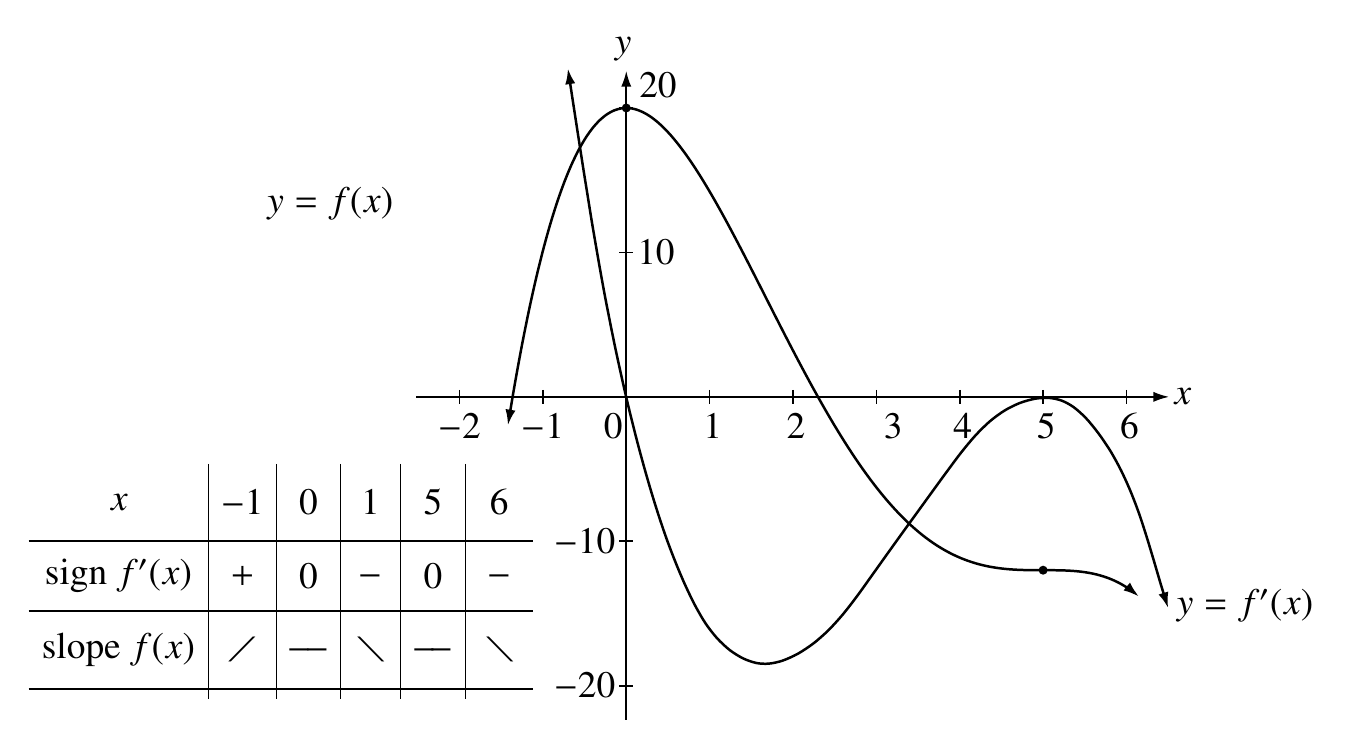
\begin{tikzpicture}[x=0.0127cm,y=-0.0127cm,font=\fontsize{13.5}{16.2}\selectfont]
\begin{scope}[shift={(386,8)}]
\draw[->] (12,370)--(765,370);
\draw[->] (222,693)--(222,44);
\draw (55.2,363)--(55.2,377);
\node at (55.2,399) {$-2$};
\draw (138.6,363)--(138.6,377);
\node at (138.6,399) {$-1$};
\node at (209.0,399) {$0$};
\draw (305.4,363)--(305.4,377);
\node at (308.4,399) {$1$};
\draw (388.8,363)--(388.8,377);
\node at (391.8,399) {$2$};
\draw (472.2,363)--(472.2,377);
\node at (489,399) {$3$};
\draw (555.6,363)--(555.6,377);
\node at (558.6,399) {$4$};
\draw (639.0,363)--(639.0,377);
\node at (642.0,399) {$5$};
\draw (722.4,363)--(722.4,377);
\node at (725.4,399) {$6$};
\draw (215,81.0)--(229,81.0);
\node[right] at (225,58) {$20$};
\draw (215,225.5)--(229,225.5);
\node[right] at (223,225.5) {$10$};
\draw (215,514.5)--(229,514.5);
\node[left] at (221,514.5) {$-10$};
\draw (215,659.0)--(229,659.0);
\node[left] at (221,659.0) {$-20$};
\node at (219,22) {$y$};
\node at (778,370) {$x$};
\draw[<->,line width=0.9pt] plot[smooth] coordinates {(163.6,41.4) (167.5,67.12) (171.4,92.57) (175.4,118.4) (179.3,143.5) (183.4,169) (187.5,194.5) (191.8,219.7) (196.2,244.8) (200.8,269.9) (205.7,294.9) (210.7,319.6) (216.1,344.5) (221.7,369.3) (227.6,393.7) (233.8,418) (240.4,442.2) (247.4,466.3) (254.9,490.2) (262.8,513.3) (271.4,535.8) (280.6,557.5) (290.7,578.4) (301.3,596.6) (312.8,611.4) (325.5,623.3) (338.8,631.6) (352,636.2) (364.4,636.9) (378,634) (393.6,627) (409.3,616.6) (424.2,603.5) (438.6,587.7) (452.7,569.6) (467.2,549.4) (482.1,528.5) (497.1,507.6) (512.4,486.5) (527.4,465.8) (542.7,444.8) (557.4,425.2) (571.5,408.4) (585.8,394.4) (600.6,383.6) (615.8,376.1) (631.2,371.8) (645.6,371.1) (657.7,373.8) (669.3,380.1) (681.8,391.2) (694.6,406.8) (706.6,424.6) (717.1,443.8) (726.4,464.3) (734.8,486.2) (742.3,509.1) (749.5,532.9) (756.8,557.7) (764.1,581.3)};
\node at (841,579) {$y=f^{\prime}(x)$};
\end{scope}
\draw[<->,line width=0.9pt] plot[smooth,domain=-1.42:6.15,samples=90] ({608+83.4*\x},{378-14.45*(20-0.6144*(\x*\x*\x*\x/4-10*\x*\x*\x/3+12.5*\x*\x))});
\fill (608,89) circle (4.5); \fill (1025,551.4) circle (4.5);
\node at (312,185) {$y=f(x)$};
\draw (10,522)--(515,522);
\draw (10,592)--(515,592);
\draw (10,670)--(515,670);
\draw (190,445)--(190,680);
\draw (258,445)--(258,680);
\draw (322,445)--(322,680);
\draw (382,445)--(382,680);
\draw (447,445)--(447,680);
\node at (100.0,483.5) {$x$};
\node at (224.0,483.5) {$-1$};
\node at (290.0,483.5) {$0$};
\node at (352.0,483.5) {$1$};
\node at (414.5,483.5) {$5$};
\node at (481.0,483.5) {$6$};
\node at (100.0,557.0) {sign $f'(x)$};
\node at (224.0,557.0) {$+$};
\node at (290.0,557.0) {$0$};
\node at (352.0,557.0) {$-$};
\node at (414.5,557.0) {$0$};
\node at (481.0,557.0) {$-$};
\node at (100.0,631.0) {slope $f(x)$};
\node at (224.0,631.0) {$\diagup$};
\node at (290.0,631.0) {$-\!-$};
\node at (352.0,631.0) {$\diagdown$};
\node at (414.5,631.0) {$-\!-$};
\node at (481.0,631.0) {$\diagdown$};\end{tikzpicture}
\end{document}
